% questions.tex —— 2001 年·春季京蒙皖卷·理科 · 题目内容片段（无答案）
% 由 tools/generate_projects.py 依来源总账自 2001/2001_数学真题_春季京蒙皖理_试题.md 生成，勿手改（改源 MD 后重跑）


\gkpart{数学}

\begin{gktip}
\textbf{来源说明}：本题面依据固定源 PDF《2001 普通高等学校春季招生考试（京蒙皖理）》两页题面逐题转录，原卷印刷页码 79–80。固定源不附答案，答案和解析均由本库独立复算。

\textbf{图形说明}：第 11、19 题的原卷图形关系重绘为 TikZ/PGFPlots 矢量图。图形标记所指的 PNG 不随仓库保存。
\end{gktip}

\gkpart{一、选择题}

\begin{question}
\gkti{1}集合 $M=\{1,2,3,4,5\}$ 的子集个数是\mbox{（　　）}

（A）$32$　　（B）$31$　　（C）$16$　　（D）$15$

\end{question}
\begin{question}
\gkti{2}函数 $f(x)=a^x$（$a>0$ 且 $a\ne1$）对于任意的实数 $x\text{、}y$ 都有\mbox{（　　）}

（A）$f(xy)=f(x)f(y)$　　（B）$f(xy)=f(x)+f(y)$

（C）$f(x+y)=f(x)f(y)$　　（D）$f(x+y)=f(x)+f(y)$

\end{question}
\begin{question}
\gkti{3}计算

\nopagebreak[4]
\[
\lim_{n\to\infty}\frac{\binom{2n}{n}}{\binom{2n+2}{n+1}}
\]

（A）$0$　　（B）$2$　　（C）$\dfrac12$　　（D）$\dfrac14$

\end{question}
\begin{question}
\gkti{4}函数 $y=-\sqrt{1-x}$（$x\le1$）的反函数是\mbox{（　　）}

（A）$y=x^2-1$（$-1\le x\le0$）　　（B）$y=x^2-1$（$0\le x\le1$）

（C）$y=1-x^2$（$x\le0$）　　（D）$y=1-x^2$（$0\le x\le1$）

\end{question}
\begin{question}
\gkti{5}极坐标系中，圆 $\rho=4\cos\theta+3\sin\theta$ 的圆心的坐标是\mbox{（　　）}

（A）$\left(\dfrac52,\arcsin\dfrac35\right)$　　（B）$\left(5,\arcsin\dfrac45\right)$

（C）$\left(5,\arcsin\dfrac35\right)$　　（D）$\left(\dfrac52,\arcsin\dfrac45\right)$

\end{question}
\begin{question}
\gkti{6}设动点 $P$ 在直线 $x=1$ 上，$O$ 为坐标原点。以 $OP$ 为直角边、点 $O$ 为直角顶点作等腰直角三角形 $OPQ$，则动点 $Q$ 的轨迹是\mbox{（　　）}

（A）圆　　（B）两条平行直线　　（C）抛物线　　（D）双曲线

\end{question}
\begin{question}
\gkti{7}已知 $f(x^6)=\log_2x$，那么 $f(8)$ 等于\mbox{（　　）}

（A）$\dfrac43$　　（B）$8$　　（C）$18$　　（D）$\dfrac12$

\end{question}
\begin{question}
\gkti{8}若 $A\text{、}B$ 是锐角三角形 $ABC$ 的两个内角，则点

\nopagebreak[4]
\[
P(\cos B-\sin A,\sin B-\cos A)
\]

在\mbox{（　　）}

（A）第一象限　　（B）第二象限　　（C）第三象限　　（D）第四象限

\end{question}
\begin{question}
\gkti{9}如果圆锥的侧面展开图是半圆，那么这个圆锥的顶角（圆锥轴截面中两条母线的夹角）是\mbox{（　　）}

（A）$30^\circ$　　（B）$45^\circ$　　（C）$60^\circ$　　（D）$90^\circ$

\end{question}
\begin{question}
\gkti{10}若实数 $a\text{、}b$ 满足 $a+b=2$，则 $3^a+3^b$ 的最小值是\mbox{（　　）}

（A）$18$　　（B）$6$　　（C）$2\sqrt3$　　（D）$2\sqrt[4]{3}$

\Needspace{0.4\textheight}
\end{question}
\begin{question}
\gkti{11}如图是正方体的平面展开图。在这个正方体中：① $BM$ 与 $ED$ 平行；② $CN$ 与 $BE$ 是异面直线；③ $CN$ 与 $BM$ 成 $60^\circ$ 角；④ $DM$ 与 $BN$ 垂直。以上四个命题中，正确命题的序号是\mbox{（　　）}
\nopagebreak[4]
\begin{center}% 2001 年春季京蒙皖卷第 11 题：正方体平面展开图
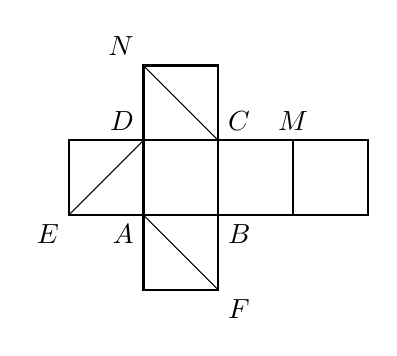
\begin{tikzpicture}[scale=0.95]
  \coordinate (A) at (0,0);
  \coordinate (B) at (1,0);
  \coordinate (C) at (1,1);
  \coordinate (D) at (0,1);
  \coordinate (E) at (-1,0);
  \coordinate (EL) at (-1,1);
  \coordinate (N) at (0,2);
  \coordinate (NT) at (1,2);
  \coordinate (F) at (1,-1);
  \coordinate (FB) at (0,-1);
  \coordinate (M) at (2,1);
  \coordinate (MR) at (2,0);
  \coordinate (RR) at (3,1);
  \coordinate (RRL) at (3,0);

  \draw[thick] (A)--(B)--(C)--(D)--cycle;
  \draw[thick] (E)--(A)--(D)--(EL)--cycle;
  \draw[thick] (D)--(C)--(NT)--(N)--cycle;
  \draw[thick] (A)--(B)--(F)--(FB)--cycle;
  \draw[thick] (C)--(M)--(MR)--(B)--cycle;
  \draw[thick] (M)--(RR)--(RRL)--(MR);
  \draw (E)--(D) (N)--(C) (A)--(F);

  \node[above left] at (N) {$N$};
  \node[above left] at (D) {$D$};
  \node[above right] at (C) {$C$};
  \node[above] at (M) {$M$};
  \node[below left] at (E) {$E$};
  \node[below left] at (A) {$A$};
  \node[below right] at (B) {$B$};
  \node[below right] at (F) {$F$};
\end{tikzpicture}
\end{center}
\nopagebreak[4]
（A）①②③　　（B）②④　　（C）③④　　（D）②③④

\end{question}
\begin{question}
\gkti{12}根据市场调查结果，预测某种家用商品从年初开始的 $n$ 个月内累积的需求量 $S_n$（万件）近似地满足

\nopagebreak[4]
\[
S_n=\frac n{90}(21n-n^2-5)\qquad(n=1,2,\cdots,12)
\]

按此预测，在本年度内，需求量超过 $1.5$ 万件的月份是\mbox{（　　）}

（A）$5$ 月、$6$ 月　　（B）$6$ 月、$7$ 月　　（C）$7$ 月、$8$ 月　　（D）$8$ 月、$9$ 月

\end{question}
\gkpart{二、填空题}

\begin{question}
\gkti{13}已知球内接正方体的表面积为 $S$，那么球体积等于\gkblank{}。

\end{question}
\begin{question}
\gkti{14}椭圆 $x^2+4y^2=4$ 长轴上一个顶点为 $A$，以 $A$ 为直角顶点作一个内接于椭圆的等腰直角三角形，该三角形的面积是\gkblank{}。

\end{question}
\begin{question}
\gkti{15}已知

\nopagebreak[4]
\[
\sin^2\alpha+\sin^2\beta+\sin^2\gamma=1
\]

（$\alpha\text{、}\beta\text{、}\gamma$ 均为锐角），那么 $\cos\alpha\cos\beta\cos\gamma$ 的最大值等于\gkblank{}。

\end{question}
\begin{question}
\gkti{16}已知 $m\text{、}n$ 是直线，$\alpha\text{、}\beta\text{、}\gamma$ 是平面，给出下列命题：

①若 $\alpha\perp\beta$，$\alpha\cap\beta=m$，$n\perp m$，则 $n\perp\alpha$ 或 $n\perp\beta$；

②若 $\alpha\parallel\beta$，$\alpha\cap\gamma=m$，$\beta\cap\gamma=n$，则 $m\parallel n$；

③若 $m$ 不垂直于 $\alpha$，则 $m$ 不可能垂直于 $\alpha$ 内的无数条直线；

④若 $\alpha\cap\beta=m$，$n\parallel m$，且 $n\not\subset\alpha$，$n\not\subset\beta$，则 $n\parallel\alpha$ 且 $n\parallel\beta$。

其中正确的命题的序号是\gkblank{}。（注：把你认为正确的命题的序号都填上）

\end{question}
\gkpart{三、解答题}

\begin{question}
\gkti{17}设函数

\nopagebreak[4]
\[
f(x)=\frac{x+a}{x+b}\qquad(a>b>0)
\]

求 $f(x)$ 的单调区间，并证明 $f(x)$ 在其单调区间上的单调性。

\end{question}
\begin{question}
\gkti{18}已知 $z^7=1$（$z\in\mathbb C$ 且 $z\ne1$）。

（1） 证明 $1+z+z^2+z^3+z^4+z^5+z^6=0$；

（2） 设 $z$ 的辐角为 $\alpha$，求 $\cos\alpha+\cos2\alpha+\cos4\alpha$ 的值。

\Needspace{0.4\textheight}
\end{question}
\begin{question}
\gkti{19}已知 $V C$ 是 $\triangle ABC$ 所在平面的一条斜线，点 $N$ 是 $V$ 在平面 $ABC$ 上的射影，且在 $\triangle ABC$ 的高 $CD$ 上。$AB=a$，$VC$ 与 $AB$ 之间的距离为 $h$，点 $M\in VC$。
\nopagebreak[4]
\begin{center}% 2001 年春季京蒙皖理卷第 19 题：斜线与三棱锥空间关系
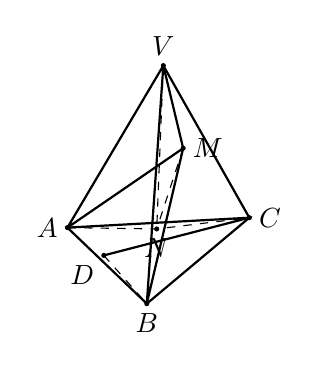
\begin{tikzpicture}[>=stealth, scale=0.84]
  \coordinate (A) at (0,0);
  \coordinate (B) at (1.2,-1.15);
  \coordinate (C) at (2.75,0.15);
  \coordinate (D) at (0.55,-0.42);
  \coordinate (N) at (1.35,-0.02);
  \coordinate (M) at (1.75,1.2);
  \coordinate (V) at (1.45,2.45);

  \draw[thick] (A)--(B)--(C)--cycle;
  \draw[thick] (C)--(D);
  \draw[dashed] (D)--(B) (A)--(N)--(C);
  \draw[thick] (V)--(C) (V)--(A) (V)--(B) (M)--(A) (M)--(B);
  \draw[dashed] (V)--(N) (M)--(N);
  \draw[thick] (V)--(M);

  \fill (A) circle (1.1pt) node[left] {$A$};
  \fill (B) circle (1.1pt) node[below] {$B$};
  \fill (C) circle (1.1pt) node[right] {$C$};
  \fill (D) circle (1.1pt) node[below left] {$D$};
  \fill (N) circle (1.1pt) node[below] {$N$};
  \fill (M) circle (1.1pt) node[right] {$M$};
  \fill (V) circle (1.1pt) node[above] {$V$};
\end{tikzpicture}
\end{center}
\nopagebreak[4]
（1） 证明 $\angle MDC$ 是二面角 $M-AB-C$ 的平面角；

（2） 当 $\angle MDC=\angle CVN$ 时，证明 $VC\perp$ 平面 $AMB$；

（3） 若 $\angle MDC=\angle CVN=\theta$（$0<\theta<\dfrac\pi2$），求四面体 $MABC$ 的体积。

\end{question}
\begin{question}
\gkti{20}在 $1$ 与 $2$ 之间插入 $n$ 个正数 $a_1,a_2,\cdots,a_n$，使这 $n+2$ 个数成等比数列；又在 $1$ 与 $2$ 之间插入 $n$ 个正数 $b_1,b_2,\cdots,b_n$，使这 $n+2$ 个数成等差数列。记

\nopagebreak[4]
\[
A_n=a_1a_2\cdots a_n,\qquad B_n=b_1+b_2+\cdots+b_n
\]

（1） 求数列 $\{A_n\}$ 和 $\{B_n\}$ 的通项；

（2） 当 $n\ge7$ 时，比较 $A_n$ 与 $B_n$ 的大小，并证明你的结论。

\end{question}
\begin{question}
\gkti{21}某摩托车生产企业，上年度生产摩托车的投入成本为 $1$ 万元/辆，出厂价为 $1.2$ 万元/辆，年销售量为 $1000$ 辆。本年度为适应市场需求，计划提高产品档次，适度增加投入成本。若每辆车投入成本增加的比例为 $x$（$0<x<1$），则出厂价相应提高的比例为 $0.75x$，同时预计年销售量增加的比例为 $0.6x$。已知年利润 $=$（出厂价$-$投入成本）$\times$年销售量。

（1） 写出本年度预计的年利润 $y$ 与投入成本增加的比例 $x$ 的关系式；

（2） 为使本年度的年利润比上年有所增加，问投入成本增加的比例 $x$ 应在什么范围内？

\end{question}
\begin{question}
\gkti{22}已知抛物线 $y^2=2px$（$p>0$）。过动点 $M(a,0)$ 且斜率为 $1$ 的直线 $l$ 与该抛物线交于不同的两点 $A\text{、}B$，$|AB|\le2p$。

（1） 求 $a$ 的取值范围；

（2） 若线段 $AB$ 的垂直平分线交 $AB$ 于点 $Q$，交 $x$ 轴于点 $N$，试求直角三角形 $NAB$ 的面积最大值。

\end{question}